\chapter{Monte Carlo Radiative Transfer and Ionization}

\epigraph{``I'm splashing greys where once was glowing white''}{{\sl Mike Vennart, Silent/Transparent}}

In the previous chapters I have given, in fairly broad brush strokes,
an introduction to the field and some relevant background relating to accretion 
discs and their associated outflows. Now it proves useful
to discuss some of the specific {\sl methods} one might be able to utilise 
in order to try and answer some of the questions raised in the previous sections.
In particular, I will discuss radiative transfer techniques and 
their potential applications.

\section{Fundamentals of Radiative Transfer}

The most fundamental quantity of radiative transfer is the 
{\em specific intensity}, $I_\nu$, defined as

\begin{equation}
I_\nu = \frac{dE}{d\Omega~dt~dA~d\nu},
\end{equation}

which has units of ${\rm erg~s^{-1}~Hz^{-1}~sr^{-1}~cm^{-2}}$.
It is useful here to also define the `moments' of the radiation field

\begin{equation}
I_\nu = 
\end{equation}

\begin{equation}
I_\nu = .
\end{equation}

The equation describing the specific intensity change along a path element $ds$
is the radiative transfer equation, 

\begin{equation}
\frac{d I_\nu}{ds} = -\kappa_\nu I_\nu + j_\nu, 
\end{equation}

where $\kappa_\nu$ and $j_\nu$ are the absorption and emission coefficients respectively.
If we define the optical depth $d \tau_\nu = \kappa_\nu ds$ we can recast this as

\begin{equation}
\frac{d I_\nu}{d \tau_\nu} = -I_\nu + S_\nu
\label{eq:formal_rte}
\end{equation}

where $S_\nu=j_\nu/\kappa_\nu$ is the source function. This equation
is called the {\em formal radiative transfer equation}, and can be solved to give 

\begin{equation}
I_\nu = I_{\nu,0}~e^{-\tau_\nu} + S_\nu (1 - e^{-\tau_\nu})
\label{eq:rte_solution}
\end{equation}

% The mean intensity, $J_\nu$ is a particularly useful quantity when calculation the ionization
% state 

\subsection{Spectral Line Formation}

From the above equations, it is trivial to show how emission and absorption lines form.
Say we have a plasma illuminated by a blackbody of temperature $T_0$, such that
$I_{\nu,0} = B_\nu (T_0)$. The plasma layer then has a different temperature, $T$,
such that $S_\nu = B_\nu (T)$ in that medium. By inspecting equation~\ref{eq:rte_solution}
we can see that if we are optically thick within the line, but optically
thin in the continuum, then inside the line the source term is dominant and outside 
the line the first $I_{\nu,0}~e^{-\tau_\nu}$ term dominates. Therefore, if $T > T_0$ we will 
see an emission line, and if $T < T_0$ we will see an absorption line. 
This approach describes line emission in the blackbody limit; for more complicated SED shapes
it is necessary to construct simple model atoms.

\subsection{The Two Level Atom}

The two level atom formalism is well described by Mihalas (1978). 


\subsubsection{Einstein Coefficients}

Within the two level atom, the rate equation between the two levels in LTE can
can be written by invoking detailed balance, such that 
\begin{equation}
B_{12} \bar{J}_{21} n_1 = B_{21} \bar{J}_{21} n_2 + A_{21} n_2,
\label{eq:rate_einstein}
\end{equation}
where $B_{12}$, $B_{21}$ and $A_{21}$ are the {\em Einstein coefficients}
for absorption, stimulated emission and spontaneous emission respectively.
In LTE, the level populations obey Boltzmann statistics, and thus we can also
write
\begin{equation}
\frac{n_1}{n_2} = \frac{g_1}{g_2} \exp (h \nu_0 / k_B T)
\end{equation}
We can then rearrange equation~\ref{eq:rate_einstein} in terms of the mean intensity,
and use the fact that, in LTE, $\bar{J}_{21} = B_\nu (T)$ to write
\begin{equation}
\bar{J}_{21} = (2 h \nu_0^3) / c^2.
\end{equation}
Since this must be true at all values of $T$ we can also show that 
\begin{equation}
A_{21} / B_{21} = (2 h \nu_0^3)~B_{12} / B_{21} = g_2 / g_1
\end{equation}



\subsubsection{Line Emission and Collisions}




\subsection{The Sobolev Approximation}

The Sobolev approximation (SA) is a useful limit originally developed.
It is used to treat line transfer in fast-moving flows. Originally 
the theory was mostly applied to Stellar winds, although since then
a wide variety of astrophysical objects have been modelled using Sobolev treatments,
such as accreting systems (this work) and Supernovae.

The Sobolev limit 



\subsubsection{Escape Probabilities}





\subsection{Monte Carlo approaches}

Simple radiation transfer problems can be solved analytically,
but with more complicated geometries it is necessary to use Monte Carlo
techniques, which are easily solved with modern computing approaches and 
are intuitively parallelisable problems. I will describe one specific 
Monte Carlo radiative transfer (MCRT) code, which has been used
for the majority of the work in this thesis.


\section{{\sc python}: A Monte Carlo Ionization and Radiative Transfer Code}

\py\footnote{Named c. 1995, predating the inexorable rise of a certain widely used
programming language.} is a Monte Carlo  ionization and radiative transfer code. 
The code has already been described extensively by LK02, SDL05 and 
Higginbottom et al. (2013; hereafter H13), so here we provide only a brief summary of its operation, 
focusing particularly on new aspects of our implementation of macro-atoms into the code.

\subsection{Basics}

\begin{figure}
\centering
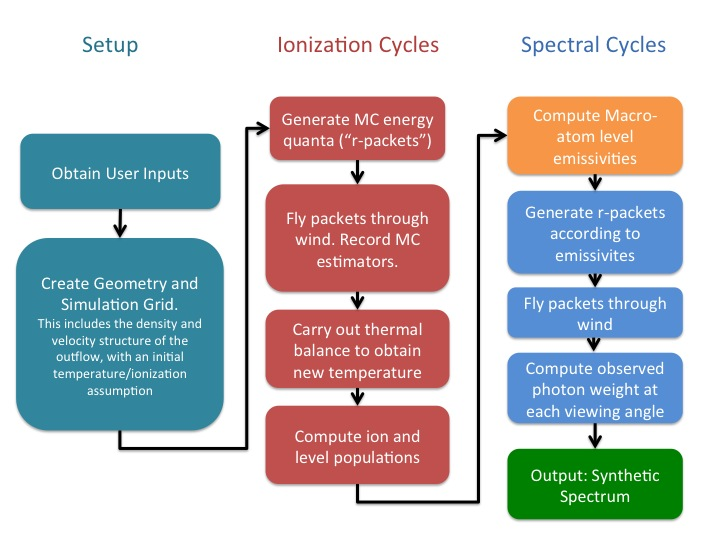
\includegraphics[width=1.0\textwidth]{figures/flowchart.jpg}
\caption
{
A flowchart showing the basic operation of \py.
} 
\label{fig:flowchart}
\end{figure}


\py\ operates in two distinct stages. First, the ionization state,
level populations and temperature structure are calculated. This is
done iteratively, by propagating several populations of Monte Carlo energy quanta (`photons')
through a model wind. The geometric and kinemetic properties of the
outflow are specified on a pre-defined spatial grid. In each of these
iterations (`ionization cycles'), the code records estimators that 
characterize the radiation field in each grid cell. At the end 
of each ionization cycle, a new electron temperature is calculated
that more closely balances heating and cooling in the 
plasma. The radiative estimators and updated electron
temperature are then used to revise the ionization state of the wind,
and a new ionization cycle is started. The process is repeated until
heating and cooling are balanced throughout the wind. 

This converged model is then used as the basis for the second set of
iterations (`spectral cycles'). In these, the emergent spectrum over
the desired spectral range is synthesized by tracking populations of
energy packets through the wind and computing the emergent spectra at
a number of user-specified viewing angles.  

\py\ is designed to operate in a number of different
regimes, both in terms of the scale of the system and in terms of the
characteristics of the underlying radiation field.
It was originally developed by LK02 in order to model the UV spectra
of CVs with a simple biconical disc wind model. SDL05
\nocite{simmacro2005} used the code to model Brackett
and Pfund line profiles of H in young-stellar objects (YSOs). As part
of this effort, they implemented a `macro-atom' mode (see below) in
order to correctly treat H recombination lines with
\py. Finally, H13 used \py\ to model broad absorption line (BAL) QSOs. For
this application, an improved treatment of ionization was implemented,
so that the code is now capable of dealing with arbitrary
photo-ionizing SEDs, including non-thermal and multi-component ones. 



\section{Macro-atoms}

{\sl The macro-atom scheme was created by Leon Lucy and is outlined in 
his 2002/03 papers. It was implemented in \py\ by Stuart Sim, initially
for the study of recombination lines in YSO (Sim et al. 2005).}

Lucy (2002, 2003\nocite{lucy2002, lucy2003}; hereafter L02, L03) 
has shown that it is possible to calculate the emissivity of a gas in
statistical equilibrium without approximation for problems with large departures
from LTE.
% accurately by quantising matter into
% `macro-atoms', and radiant and kinetic energy into indivisible energy
% packets (r- and k- packets, respectively). 
His macro-atom scheme allows for all possible transition paths from a given level,
dispending with the two-level approximation, and
provides a full non-local thermodynamic equilibrium (NLTE) solution
for the level populations based on Monte Carlo estimators. The macro-atom
technique has already been used to model Wolf-Rayet star
winds \citep{sim2004}, AGN disc winds \citep{simlong2008, tatum2012},
supernovae \citep{kromersim2009, kerzendorfsim} and YSOs (SDL05). A full 
description of the approach can be found in L02 and L03. 

The fundamental approach here requires somewhat of a philosophical shift.
Normally MCRT is described in the most intuitive way- that is, we imagine
real photons striking atoms and scattering, or photoionizing 
and depositing energy in a plasma. With Lucy's scheme one should instead 
reimagine the MC quanta as a packets of quantised energy flow, and the scheme as a 
{\em statistical} one. The amount of time a given energy quanta spends in a specific atomic
level or thermal pool is then somewhat analogous to the absolute energy 
contained therein.

Following L02, let us consider an atomic species interacting with a radiation field.
If the quantity $\epsilon_j$ represents the ionization plus excitation energy of 
a level i then the rates at which the level $j$ absorbs and emits radiant energy 
are given by

\begin{equation}
 \dot{A}_{j}^{R} = R_{\ell j} \epsilon_{j \ellp} \;\;\;\;\; and \;\;\;
\;\;  \dot{E}_{i}^{R} = R_{j \ellp} \epsilon_{j \ellp} \;\;\; ,
\end{equation}

Where we adopt Lucy's convention in which the subscript $\ellp$ denotes a summation over
all lower states.
Similarly, the rates corresponding to {\em kinetic} energy transport can then be written as

\begin{equation}
 \dot{A}_{j}^{C} = C_{\ellp j} \epsilon_{j \ellp} \;\;\;\;\; and
\;\;\;
\;\;  \dot{E}_{j}^{C} = C_{j \ellp} \epsilon_{j \ellp} \;\;\; ,
\end{equation}

If we now impose statistical equilibrium
%
\begin{equation}
 ({\cal R}_{\ellp j}-{\cal R}_{j \ell})+({\cal R}_{uj}-{\cal R}_{ju})=0 \;\;\;.
\end{equation}
 
we can then obtain 

\begin{eqnarray}
 \dot{E}_{j}^{R}+\dot{E}_{j}^{C}+{\cal R}_{ju}\epsilon_{i}+
 {\cal R}_{j \ell}\epsilon_{\ell}  \nonumber \\  
 = \dot{A}_{j}^{R}+\dot{A}_{j}^{C}+{\cal R}_{uj} \epsilon_{i}
 +{\cal R}_{\ell j} \epsilon_{\ell}           .  
 \label{eq:matom_SE}     
\end{eqnarray}

This equation is the starting point for the macro-atom scheme. It shows 
that, when assuming only radiative equilibrium, the energy flows through
a system depend only on the transition probabilities and atomic physics
associated with the levels the energy flow interacts with.
By quantising this energy flow into radiant (r-) and kinetic (k-) packets, 
we can simulate the energy transport through
a plasma discretised into volume elements (``macro-atoms''),
whose associated transition probabilities govern the interaction 
of radiant and kinetic energy with the ionization and excitation energy associated 
with the ions of the plasma.

Although equation~\ref{eq:matom_SE} assumes strict radiative equilbrium,
it is trivial to adjust it to include non-radiative source and sink terms. 
For example, in an expanding parcel of plasma, adiabatic cooling may be 
included with a simple modification to the RHS of equation~\ref{eq:matom_SE}.
%% XXX CHECK THIS.

% \subsection{Superlevels}
% One undesirable aspect of the macro-atom scheme is that the number of 
% jumps made inside a macro-atom can become large in certain limits.
% For example, when the plasma starts to approach LTE conditions
% the energy packets will spend a huge amount of time
% jumping between high up levels in a macro-atom. Fortunately, there
% are a number of fairly elegant solutions here. The first would be simply 
% to keep track of net rates-- if two large rates go in opposite directions
% but have a net difference, then all one needs to do is take account of that net
% difference and set the other rate to zero. This could be implemented in \py\, but
% is not currently. Instead, we adopt a method I shall refer to using the 
% term `superlevels'. 

% Once a cycle has been computed, it is possible to calculate departure coefficients, $D_j$
% for a level $j$, which are defined as

% \begin{equation}
% D_j = \frac{n_j}{n_j^{*,T_e}},
% \end{equation}

% which is simply the ratio of a level's population to it's LTE population at the electron temperature.
% If these coefficients approach unity at all levels above some threshold then these
% levels are said to be part of a superlevel. Any time we jump to a level $j$ inside a superlevel
% we instantly select a new level $k$ with a probability

% \begin{equation}
% P(j,k) = \frac{1}{N} \frac{n_j^{*,T_e}}{g_k} \sum_l P(k,l),
% \end{equation}
 
% where $1/N$ is just a normalisation over the sum of these quantities and $\sum_l P(k,l)$ represents 
% the sum of jumping probabilities to lower levels below the superlevel threshold.
% This formula produces the required jumping and deactivation distributions in the limit of LTE
% without having to actually go through the lengthy process of MC sampling the probability space.
% The speed-up can be huge in certain limits-- some models can undergo $\sim10^8$ jumps before deactivation,
% compared to an average of $\sim2$ in Lucy's original simulations.

\subsection{Macro-Atom Estimators}

\subsubsection{Radiation Field Estimators}

\subsubsection{Heating And Cooling Estimators}

\subsection{Ionization Fractions and Level Populations}




\section{Simple-atoms}

% Prior to SDL05, the relative ionization fractions for all atomic
% species were estimated via the modified Saha equation (Mazzali \&
% Lucy 1993)  
% \begin{equation}
% \frac{n_{j+1} n_e}{n_j} = W [\xi + W(1-\xi)]
% \left(\frac{T_e}{T_R}\right)^{1/2}
% \left(\frac{n_{j+1}n_e}{n_j}\right)^*_{T_R}. \label{ionization}
% \end{equation}
% Here, the `starred' term on the right represents abundances computed with
% the Saha equation at temperature $T_R$, but using partition functions
% from the dilute blackbody approximation. 
% $W$ is an effective dilution factor, $\xi$ is the
% fraction of recombinations going directly to the ground state, and
% $T_R$ and $T_e$ are the radiation and electron temperatures,
% respectively. This simple ionization scheme produces reasonable
% results when the photoionizing SED can be approximated by a dilute
% blackbody. This is the case for high-state CVs. (As noted above, an
% improved, but more complex treatment of ionization that is appropriate
% for more complex SEDs is described in H13.) 

% Similarly, the relative excitation fractions within each ionization
% stage of a given species were estimated via a modified (dilute) Boltzmann
% equation,
% \begin{equation}
% \frac{n_{jk}}{n_j} = \frac{W g_k}{z_j(T_R)} \exp(-E_k/kT_R),
% \end{equation}
% where $n_{jk}$ is the population of level $k$ in ionic stage $j$,
% $E_k$ is the energy difference between level $k$ and the ground state,
% $g_k$ is the statistical weight of level $k$
% and $z_j(T_R)$ is the partition function of ionic stage $j$. 
% This equation is approximate, and in general this approximation 
% is not good. We therefore endeavour to treat any species in
% which the excitation state of the ions is thought to be important
% in determining either the ionizing radiation field, or emergent spectrum,
% as macro-atoms.

% Finally, \py\ originally modelled all bound-bound processes as transitions
% within a simple two-level atom \cite[e.g.][]{mihalas}. 
% This framework was used for the treatment of line transfer and also
% for the line heating and cooling calculations (see LK02). 
% The approximation works reasonably well for resonance  
% lines, such as \civfull, in which the lower level is the ground state.  
% However, it is a poor approximation for many other
% transitions, particularly those where the upper level
% is primarily populated from above. Thus an improved method for
% estimating excited level populations and simulating line transfer is
% needed in order to model recombination lines and continua.

\section{Heating And Cooling}

\subsection{Heating And Cooling Balance}

\subsection{Heating And Cooling Estimators}


Here I've tried to use Lucy's notation for macro-atom estimators. Take a three level system, in
which $l$ and $u$ represent lower and upper levels, 
and $\kappa$ represents the continuum level or upper ion.
q is the `absorption fraction' derived below, and $q_{ul}$ and $q_{lu}$ are the collisional
rate coefficients.

\subsubsection{Macro-atoms}

\noindent
In the macro-atom approach, we basically treat two communication pathways.
bound-free transitions represent a way
for radiant energy to communicate with the thermal pool
and bound-bound transitions represent a way
for excitation energy to communicate with the thermal pool.
\bigskip

\noindent
The heating and cooling rates for macro-atom bound-bound transitions are the rates of
collisional excitations and de-excitations
- i.e. the rate at which thermal energy is converted into
bound-bound excitation energy and vice versa.

\begin{equation}
C_{bb,matoms} = \sum_{lines} q_{lu} n_l n_e h \nu_{ul} V
\end{equation}

\begin{equation}
H_{bb,matoms} = \sum_{lines} q_{ul} n_u n_e h \nu_{ul} V
\end{equation}

\noindent
For bound-free transitions, we define the normal photoionization and recombination
rate coefficients $\gamma$ and $\alpha$, where $\alpha$ includes
stimulated recombination as we do in the code. Note
this differs to the approach in Lucy (2003), where it is instead included as a 
negative photoionization term, hence the notation $\widetilde{\gamma}$.
We also need to define two `modified rate coefficients' which 
are the rates at which b-f transitions add and remove energy to the radiation field.
These are denoted $\gamma^E$ and $\alpha^E$.

The rate at which recombinations convert
thermal {\em and} ionization energy into radiant energy is then
$\alpha^E h\nu_{\kappa l} n_\kappa n_e$, where $h \nu_{\kappa l}$ is the potential of the 
b-f transition, or the energy difference between continuum $\kappa$ and 
the level $l$ we are recombining too. 
The amount of this energy which is removed from the actual thermal pool
therefore needs a quantity $\alpha h\nu_{\kappa l} n_\kappa n_e$ subtracted from it,
giving
\begin{equation}
C_{bf,matoms} = \sum_{bf jumps} (\alpha^E - \alpha) n_e n_{\kappa}\nu_{\kappa l} V 
\end{equation}
where here I have also included stimulated recombination as we do in the code. Note
this differs to the approach in Lucy (2003), where it is instead included as a 
negative photoionization term, hence the notation $\widetilde{\gamma}$.
For photoionizations, we write a similar expression. The rate of at which
a level $l$ absorbs energy by b-f transitions is given by $\gamma^E h\nu_{\kappa l} n_\kappa n_e$,
but the amount $\gamma h \nu_{\kappa l} n_l$ goes into ionization energy, giving 
\begin{equation}
H_{bf,matoms} = \sum_{bf jumps} (\gamma^E - \gamma) n_l h \nu_{\kappa l} V
\end{equation}
as the rate at which radiant energy heats the plasma via b-f transitions.




\subsubsection{Simple-atoms}
\noindent
In simple-ions it is in some ways a little more complicated. 
First we define $q$ which will be different for each b-b transition, 
following Nick's thesis, which is given by 
(NB: I don't actually know how to derive this)
\begin{equation}
q = \frac{q_{ul} n_e (1 - e^{-h\nu/kT_e})}{\beta_{ul} A_{ul} + q_{ul} n_e (1 - e^{-h\nu/kT_e})}
\end{equation}
where $\beta_{ul}$ is the angle-averaged escape probability. 
$q$ represents {\em the probability that an excited bound electron
will collisionally de-excite}.
Our b-b heating rate is computed during the photon propagation and is a sum
over photons which come into resonance with each line, given by 
\begin{equation}
H_{bb,simple} = \sum_{photons} \sum_{lines} (1 - q) (1 - e^{-\tau_S}) w_{photon}
\end{equation}
And our bound bound cooling rate is given by 
\begin{equation}
C_{bb,simple} = \sum_{lines} q \left(n_l\frac{g_u}{g_l} - n_u\right) q_{ul} n_e 
\frac{(1 - e^{-h\nu/kT_e})}{(e^{h\nu/kT_e} - 1)}  h \nu_{ul}
\end{equation}
%%note the difference to the macro-atom approach- here this is already 
\noindent
The bound-free heating rate is given by
\begin{equation}
H_{bf,simple} = \sum_{photons} \sum_{bfjumps} w_{photon} e^{-\tau} \frac{\nu - \nu_{0}}{\nu}
\end{equation}
where $\nu$ here is the frequency of the photon in question, and $\nu_{0}$.
The bound-free cooling rate is then

\begin{equation}
C_{bf,simple} = ??
%%\sum_{bfjumps} \alpha_{sp} n_e n_{\kappa}
\end{equation}













\section{Spectral Synthesis}

The primary output from \py\ is a synthetic spectrum 
across a range of viewing angles. 
The code utilises a variance reduction technique in order to minimise the amount of 
time spent in the portion of the code.















\section{Clumping}

\subsection{Motivation}

Clumping is often invoked in a number of different types of outflow
to explain everything from X-ray variability to 


\subsection{Microclumping}

To take account of clumping in our outflow we adopt a simple parameterization
used in stellar wind modelling. The key assumption here is that typical clump sizes
are much smaller than the typical photon mean free path, and thus the clumps are 
both geometrically and optically thin. This approach is typically 
known as microclumping and allows one to introduce a `filling factor', $f$, which is the 
fraction of the volume of the plasma filled by clumps. We can then introduce the 
`density enhancement', $D$, which is simply 

\begin{equation}
D = \frac{1}{f}
\end{equation}

The densities in the model are then multiplied by this factor. This has the effect 
of enhancing `$\rho^2$' processes such as recombination or collisional excitation,
and 


\section{Code Validation}

The main challenge for high performance scientific computing can be 
elegantly summarised by Ferland's (2002) epitaph, `Reliability in the face 
of complexity'. We have already delved into some of the complexity in this case,
so it is important to assess whether our code effectively 

\subsection{Testing against Cloudy}


\subsection{Testing against Tardis}




